\documentclass[12pt, a4paper]{article} 
 
\usepackage[utf8]{inputenc}
 

\usepackage[bottom = 8em]{geometry} % to change the page dimensions
\geometry{a4paper} % or letterpaper (US) or a5paper or....
 
\usepackage{graphicx} % support the \includegraphics command and options
\usepackage{grffile}
 
\usepackage{booktabs} % for much better looking tables
\usepackage{array} % for better arrays (eg matrices) in maths
\usepackage{float}
\usepackage{paralist} % very flexible & customisable lists (eg. enumerate/itemize, etc.)
\usepackage{verbatim} % adds environment for commenting out blocks of text & for better verbatim
\usepackage{subfig} % make it possible to include more than one captioned figure/table in a single float
% These packages are all incorporated in the memoir class to one degree or another...
 
 
 
\usepackage{amsmath, amssymb}% for mathematical symbols
\usepackage[colorlinks=true,linkcolor=black]{hyperref} % for hyperreferences with black color
%\usepackage[T1]{fontenc} % Uncomment for norwegian document
%\usepackage[norsk]{babel} %
 
%%% HEADERS & FOOTERS
\usepackage{fancyhdr} % This should be set AFTER setting up the page geometry
\pagestyle{fancy} % options: empty , plain , fancy
\renewcommand{\headrulewidth}{0pt} % customise the layout...
\lhead{}\chead{}\rhead{}
\lfoot{}\cfoot{\thepage}\rfoot{}

 
%%% SECTION TITLE APPEARANCE
\usepackage{sectsty}
\allsectionsfont{\sffamily\mdseries\upshape} % (See the fntguide.pdf for font help)
% (This matches ConTeXt defaults)
 
%%% ToC (table of contents) APPEARANCE
\usepackage[nottoc,notlof,notlot]{tocbibind} % Put the bibliography in the ToC
\usepackage[titles,subfigure]{tocloft} % Alter the style of the Table of Contents
\renewcommand{\cftsecfont}{\rmfamily\mdseries\upshape}
\renewcommand{\cftsecpagefont}{\rmfamily\mdseries\upshape} % No bold!
 
 
%%% END Article customizations
 
%%% The "real" document content comes below...
 
\title{Subsymbolic AI assignment 1}
\author{Eivind Hærum \& \ Hong-Dang Lam}
\date{\today} % Activate to display a given date or no date (if empty),
         % otherwise the current date is printed 
 
\begin{document}
\pagenumbering{gobble}
\maketitle
%\begin{abstract}
% 
%Abstract
% 
%\end{abstract}
\newpage

\tableofcontents
\pagenumbering{roman}
\newpage

\section{Implementation of the proposed system}
\pagenumbering{arabic}
Modifications and translation of the provided code etc.

\subsection{System}
The system consist of a webots simulation which uses a world file provided by the course stab. The world file consists of a food-box inside a closed square arena (4 walls) with 7 e-pucks. The box is emitting light to act as a food source, and there is also another global directional light to make the world more visible.


The underlying controller-logic for controlling the epucks is largely based upon the provided framework, where we have made some changes in epuck\_basic to have access to features such as led lights and the light sensors. We also altered search, retrieval and stagnation in our attempt to solve the task more effectively. Finally swarm\_controller is where most of our own logic is consolidated that makes use of all the functions and logic in the other files. 

The changes we made to the world file was dimming the directional light a bit so the e-puck bots would be more sensitive to the light emitted from the food source, and we changed the attenuation of the box. The attenuation of a point light is calculated as such: $ att = \frac{1}{x+y*r+z*r^2} $ where $r$ is the distance to the emitter. We changed the value of $x$ to 0 and $z$ to 6 - this is because according to the documentation it is recommended to change default attenuation to $[0,0,4\pi]$ which is more realistic in a real world scenario, but $4\pi$ is too high for the bots to efficiently find the light source, thus we settled for half the suggested value.  
\subsection{Box pushing}
%Implement control system for the box pushing task as provided in the assignment text and
%describe the expected and unexpected behaviours observed during simulation.
The bots uses the distance sensor in the search behavior where they walk aimlessly around searching for the food source. Whenever they see the box/food in front of them they will start the retrieval behavior which uses the light sensors to locate the box (this is possible because it is emitting light). The light sensors reports lower values if the closer it gets to a stronger light, and higher values otherwise.

The e-pucks only uses the light sensor [0,1,6,7] which are the four sensors in front of it. We are using the different behaviours for this assignment, search, retrieval and stagnation as provided in the .c files, but that we translated into python code. 
The search behaviour makes the bot search aimlessly around without colliding into the other bots, while retrieval will make the bot converge to the box if it can find it. After the converging is done the retrieval behaviour intiates a push box behaviour. If the bot is stuck pushing the box for a while without any results it will use stagnation to attempt to realign itself so the pushing becomes more effective. If it has tried to realign two times a "find new spot" command is issued. This makes the bot drive in a sequence of moves to let it find the side of the box to either the left or the right of its current position.
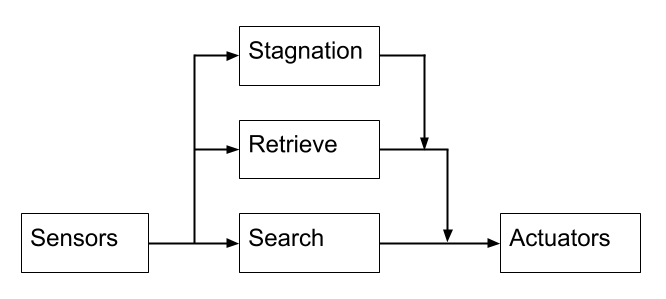
\includegraphics[width=\linewidth]{Brooks-lite.png}


We expected the bots to find the box relatively fast and then push it to the wall. This happened in certain runs, but some of them took longer than other depending on when and how the bots converged to the box. Sometimes they pushed the box in a circular motion before they were able to push it to the wall.
Unexpected results we encountered was e-puck tipping each other or the food box when clumping together for the task.\\
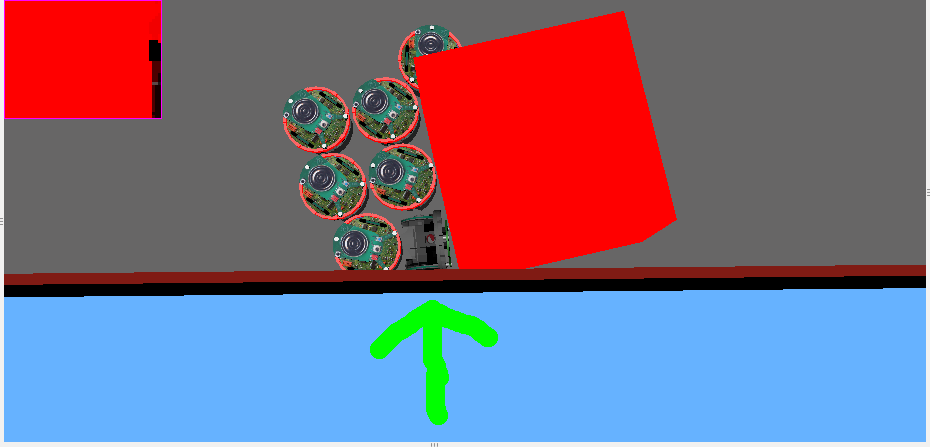
\includegraphics[width=\linewidth]{1.mandown.png}

\section{Improvements}
\subsection{Discovered weaknesses}
 %Identify areas of the system that may be improved in the single box scenario. These areas may be in overall architecture of controller or at the individual sub-behaviour task. Provide suggestions (one or more) to address these improvements

The stagnation file provided doesn't differentiate between whether the bot is close to the box or not - this led to the bots trying to find new spot before it even reached the box. We had to check this ourselves by using the distance sensors in the front. 

The bots doesn't always accomplish the mission either, they tend to get stuck now and then. This usually happens when there's two or three bots on both opposite side of the box. Both "team" think they are pushing the box, and they trust their neighbours. 
In the start we decided to try to find the box by using the camera (because the food source is the only object that is red), however there's red colors in the grey floor and on the led of the e-puck bots too. The camera approach didn't work as well as we had hoped it would, so we decided to scrap it.
The bots could also be trapped either inside a swarm of e-pucks or between the box and the wall.

The bots only have three behaviours established so they don't know if the box has reached its location or not. This makes it so the bots runs for ever even though they've accomplished the task.

It would be very helpful if the epucks had a larger sense of self, and knew for example whether it had travelled a certain distance instead of assuming that the commands its given takes it there. This would allow it to make better decisions. During the stagnation process for example the bots used the search class to determine if it is colliding with someone or something, and thus takes evasive maneuvers. This brings the bot to a place other than where it assumes it, which means that the set of commands it follows that is engineered to perform a certain sequence of moves will take it somewhere else then planned. Had the bot known how to properly handle this information, and understood the importance of location, the outcome could always turn out the same, as the bot would correct itself whenever something unanticipated happend. 

One way of handling this would be to have the robots keep a map of where it has been and thus make it easier to tell if it has deviated from its course. 



\subsection{Results from the changes made}
When we implemented the distance checking before changing to stagnation behavior it was able to push the box into the wall. We also implemented a counter for each bot, which counts how many times it believes that the pushing is not working. The first two times it will try to realign itself to it is perpendicular to the box, but if it still believes that it's not able to push the box it will start to find a new spot. This is done by reversing, turn 90$^{\circ}$, drive forward, turn 90$^{\circ}$ the other way, drive forward again, and turn towards the box. \\
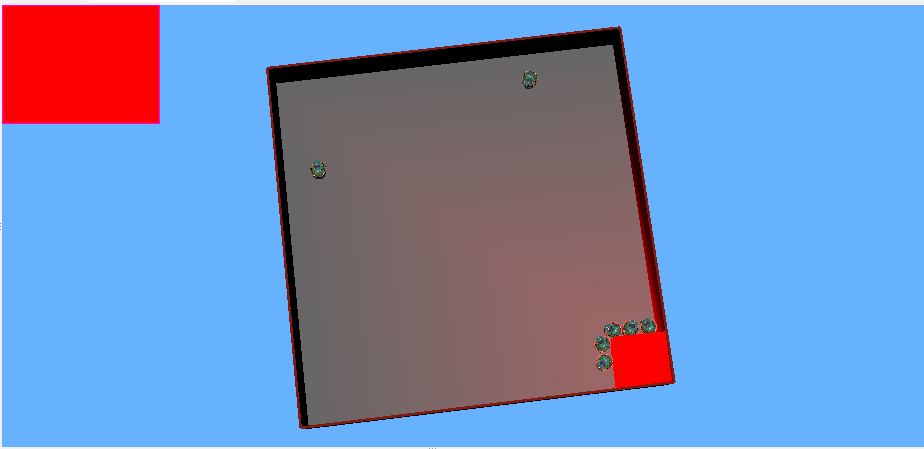
\includegraphics[width=\linewidth]{1.finalState}

We decided to scrap the camera approach for locating the box and use the retrieval.c file provided (translated to python). This "new" approach uses lightsensor to converge to the box, which is more effective because the bot can use more sensors to get a certain idea where the box is located. The camera approach could easily pick up noise from for example the other bots and the floor (because gray color contains red as well).

The way we decided to handle the problem with epuck location was to ignore collisions, so the bots would just keep on driving in the given pattern even if there were other bots in the way. This increased the probability of it being able to reach the destination it aimed for. However sometimes it's not possible to drive in the given pattern if there's obstacles along the way, meaning that the bots sometimes just stand still whilst trying to move to another position.\\

\section{Advanced features}
%TODO

\subsection{New architecture}
\subsection{Modifications}


\end{document}
